% Code inspired by https://tex.stackexchange.com/questions/243740/print-double-sided-playing-cards

\documentclass[a4paper]{article}
\usepackage{graphicx}
\usepackage[export]{adjustbox}
%\usepackage{color}
\usepackage{amsmath, amssymb}
\usepackage{tikz}
\usetikzlibrary{patterns, shadows, positioning}
\usetikzlibrary{shapes.geometric}
%\usepackage{pifont}
\usepackage{fourier-orns}
\usepackage[hmargin=0mm,vmargin=0mm, letterpaper]{geometry}
\usepackage{tabularx}
\usepackage{epsdice}

%\setlength{\parindent}{0cm}

\definecolor{titlebg}{rgb}{30, 30 , 30}

% https://latexcolor.com/
\definecolor{capri}{rgb}{0.0, 0.75, 1.0}
\definecolor{royalazure}{rgb}{0.0, 0.22, 0.66}
\definecolor{lightskyblue}{rgb}{0.53, 0.81, 0.98}

%   TikZ/PGF Settings für die Karten
\def\cardwidth{2.5in}
\def\cardheight{3.5in}

\def\ruleswidth{2in}

\def\shapeCard{(0,0) rectangle (\cardwidth, \cardheight)}

\tikzset{%
  square/.style={regular polygon,regular polygon sides=4}
}

\newcommand{\threetiles}[2]{
\begin{tikzpicture}

  \draw[black] \shapeCard;

  \filldraw[#1,draw=black]
  (0.1*\cardwidth,    0.1*\cardwidth)
  -- (0.3*\cardwidth, 0.1*\cardwidth)
  -- (0.3*\cardwidth, 0.1*\cardwidth+0.2*\cardwidth)
  -- (0.1*\cardwidth, 0.1*\cardwidth+0.2*\cardwidth)
  -- cycle;          

  \filldraw[#1,draw=black]
  (0.4*\cardwidth,    0.1*\cardwidth)
  -- (0.6*\cardwidth, 0.1*\cardwidth)
  -- (0.6*\cardwidth, 0.1*\cardwidth+0.2*\cardwidth)
  -- (0.4*\cardwidth, 0.1*\cardwidth+0.2*\cardwidth)
  -- cycle;          

  \filldraw[#1,draw=black]
  (0.1*\cardwidth,    0.4*\cardwidth)
  -- (0.3*\cardwidth, 0.4*\cardwidth)
  -- (0.3*\cardwidth, 0.4*\cardwidth+0.2*\cardwidth)
  -- (0.1*\cardwidth, 0.4*\cardwidth+0.2*\cardwidth)
  -- cycle;          

  \filldraw[#2,draw=black]
  (0.7*\cardwidth,    \cardheight-0.1*\cardwidth)
  -- (0.9*\cardwidth, \cardheight-0.1*\cardwidth)
  -- (0.9*\cardwidth, \cardheight-0.3*\cardwidth)
  -- (0.7*\cardwidth, \cardheight-0.3*\cardwidth)
  -- cycle;          
  
\end{tikzpicture}}

\newcommand{\pairtiles}[2]{
\begin{tikzpicture}

  \draw[black] \shapeCard;

  \filldraw[#1,draw=black]
  (0.1*\cardwidth,    0.1*\cardwidth)
  -- (0.3*\cardwidth, 0.1*\cardwidth)
  -- (0.3*\cardwidth, 0.1*\cardwidth+0.2*\cardwidth)
  -- (0.1*\cardwidth, 0.1*\cardwidth+0.2*\cardwidth)
  -- cycle;          

  \filldraw[#1,draw=black]
  (0.4*\cardwidth,    0.1*\cardwidth)
  -- (0.6*\cardwidth, 0.1*\cardwidth)
  -- (0.6*\cardwidth, 0.1*\cardwidth+0.2*\cardwidth)
  -- (0.4*\cardwidth, 0.1*\cardwidth+0.2*\cardwidth)
  -- cycle;          

  \filldraw[#2,draw=black]
  (0.4*\cardwidth,    \cardheight-0.1*\cardwidth)
  -- (0.6*\cardwidth, \cardheight-0.1*\cardwidth)
  -- (0.6*\cardwidth, \cardheight-0.3*\cardwidth)
  -- (0.4*\cardwidth, \cardheight-0.3*\cardwidth)
  -- cycle;          

  \filldraw[#2,draw=black]
  (0.7*\cardwidth,    \cardheight-0.1*\cardwidth)
  -- (0.9*\cardwidth, \cardheight-0.1*\cardwidth)
  -- (0.9*\cardwidth, \cardheight-0.3*\cardwidth)
  -- (0.7*\cardwidth, \cardheight-0.3*\cardwidth)
  -- cycle;          
  
\end{tikzpicture}}

\newcommand{\twotiles}[3]{
\begin{tikzpicture}

  \draw[black] \shapeCard;

  \filldraw[#1,draw=black]
  (0.1*\cardwidth,    0.1*\cardwidth)
  -- (0.3*\cardwidth, 0.1*\cardwidth)
  -- (0.3*\cardwidth, 0.1*\cardwidth+0.2*\cardwidth)
  -- (0.1*\cardwidth, 0.1*\cardwidth+0.2*\cardwidth)
  -- cycle;          

  \filldraw[#1,draw=black]
  (0.4*\cardwidth,    0.1*\cardwidth)
  -- (0.6*\cardwidth, 0.1*\cardwidth)
  -- (0.6*\cardwidth, 0.1*\cardwidth+0.2*\cardwidth)
  -- (0.4*\cardwidth, 0.1*\cardwidth+0.2*\cardwidth)
  -- cycle;          

  \filldraw[#2,draw=black]
  (0.4*\cardwidth,    \cardheight-0.1*\cardwidth)
  -- (0.6*\cardwidth, \cardheight-0.1*\cardwidth)
  -- (0.6*\cardwidth, \cardheight-0.3*\cardwidth)
  -- (0.4*\cardwidth, \cardheight-0.3*\cardwidth)
  -- cycle;          

  \filldraw[#3,draw=black]
  (0.7*\cardwidth,    0.75*\cardheight)
  -- (0.9*\cardwidth, 0.75*\cardheight)
  -- (0.9*\cardwidth, 0.75*\cardheight-0.2*\cardwidth)
  -- (0.7*\cardwidth, 0.75*\cardheight-0.2*\cardwidth)
  -- cycle;          
  
\end{tikzpicture}}

\newcommand{\onetiles}[4]{
\begin{tikzpicture}

  \draw[black] \shapeCard;

  \filldraw[#1,draw=black]
  (0.1*\cardwidth,    0.25*\cardheight)
  -- (0.3*\cardwidth, 0.25*\cardheight)
  -- (0.3*\cardwidth, 0.25*\cardheight+0.2*\cardwidth)
  -- (0.1*\cardwidth, 0.25*\cardheight+0.2*\cardwidth)
  -- cycle;          

  \filldraw[#2,draw=black]
  (0.4*\cardwidth,    0.1*\cardwidth)
  -- (0.6*\cardwidth, 0.1*\cardwidth)
  -- (0.6*\cardwidth, 0.1*\cardwidth+0.2*\cardwidth)
  -- (0.4*\cardwidth, 0.1*\cardwidth+0.2*\cardwidth)
  -- cycle;          

  \filldraw[#3,draw=black]
  (0.4*\cardwidth,    \cardheight-0.1*\cardwidth)
  -- (0.6*\cardwidth, \cardheight-0.1*\cardwidth)
  -- (0.6*\cardwidth, \cardheight-0.3*\cardwidth)
  -- (0.4*\cardwidth, \cardheight-0.3*\cardwidth)
  -- cycle;          

  \filldraw[#4,draw=black]
  (0.7*\cardwidth,    0.75*\cardheight)
  -- (0.9*\cardwidth, 0.75*\cardheight)
  -- (0.9*\cardwidth, 0.75*\cardheight-0.2*\cardwidth)
  -- (0.7*\cardwidth, 0.75*\cardheight-0.2*\cardwidth)
  -- cycle;          
  
\end{tikzpicture}}

\newcommand{\marketcard}[4]{
\begin{tikzpicture}

  \draw[black] \shapeCard;

  \filldraw[#1,draw=black]
  (0.2*\cardwidth,    0.25*\cardheight)
  -- (0.4*\cardwidth, 0.25*\cardheight)
  -- (0.4*\cardwidth, 0.25*\cardheight+0.2*\cardwidth)
  -- (0.2*\cardwidth, 0.25*\cardheight+0.2*\cardwidth)
  -- cycle;          

  \filldraw[#2,draw=black]
  (0.6*\cardwidth,    0.25*\cardheight)
  -- (0.8*\cardwidth, 0.25*\cardheight)
  -- (0.8*\cardwidth, 0.25*\cardheight+0.2*\cardwidth)
  -- (0.6*\cardwidth, 0.25*\cardheight+0.2*\cardwidth)
  -- cycle;          

  \filldraw[#3,draw=black]
  (0.2*\cardwidth,    0.75*\cardheight)
  -- (0.4*\cardwidth, 0.75*\cardheight)
  -- (0.4*\cardwidth, 0.75*\cardheight-0.2*\cardwidth)
  -- (0.2*\cardwidth, 0.75*\cardheight-0.2*\cardwidth)
  -- cycle;          

  \filldraw[#4,draw=black]
  (0.6*\cardwidth,    0.75*\cardheight)
  -- (0.8*\cardwidth, 0.75*\cardheight)
  -- (0.8*\cardwidth, 0.75*\cardheight-0.2*\cardwidth)
  -- (0.6*\cardwidth, 0.75*\cardheight-0.2*\cardwidth)
  -- cycle;          
  
\end{tikzpicture}}



\newcommand{\playercard}{
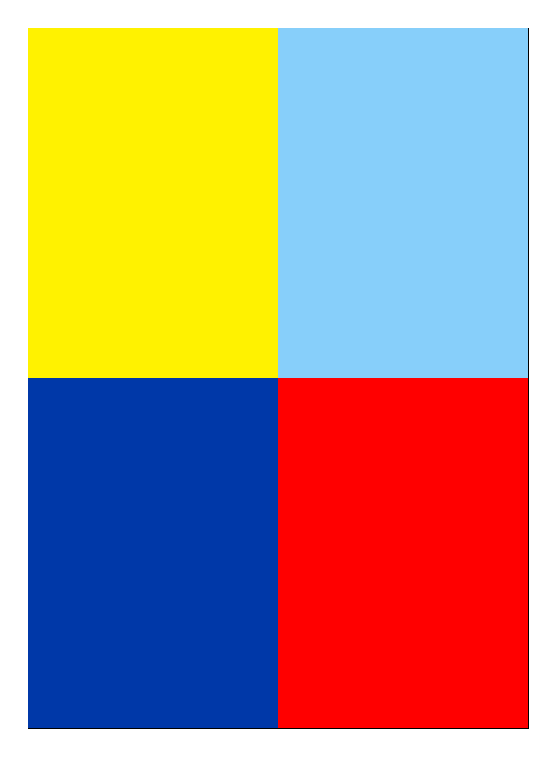
\begin{tikzpicture}
  %begin card creation

      %\draw [step=.5, help lines] (0,0) grid (\cardwidth,\cardheight);
%    % draw card boundries and clip corners
    \draw[black] \shapeCard;

    \fill[royalazure] (0,0) -- (0,\cardheight/2) -- (\cardwidth/2, \cardheight/2) -- (\cardwidth/2, 0) -- cycle;
    \fill[red]  ((\cardwidth/2,0)  -- (\cardwidth,0)     -- (\cardwidth,\cardheight/2)        -- (\cardwidth/2, \cardheight/2) -- cycle;
    \fill[yellow]    (0,\cardheight/2) -- (0,\cardheight) -- (\cardwidth/2,\cardheight)  -- (\cardwidth/2, \cardheight/2) -- cycle;
    \fill[lightskyblue]  (\cardwidth/2,\cardheight/2)  -- (\cardwidth/2,\cardheight)  -- (\cardwidth,\cardheight) -- (\cardwidth, \cardheight/2) -- cycle;
     
\end{tikzpicture}}

\newcommand{\rulescard}[1]{
\begin{tikzpicture}

  \draw[black] \shapeCard;

  \node[below right] at (0.1*\cardwidth,\cardheight-0.1*\cardwidth) {#1};
   
\end{tikzpicture}}


\begin{document}

% https://tex.stackexchange.com/questions/56101/spaces-between-rows-and-cols-in-a-table-better-ways-than-mine
\setlength\tabcolsep{0pt}
\renewcommand{\arraystretch}{0}

\begin{table}[h]
  \centering
  \begin{tabular}{|c|c|c|}
    \rulescard {
      \begin{minipage}[t]{\ruleswidth}
        
        \textbf{Draft phase}: Randomly draw 4 tile cards with market
        side up. Players draft a tile card in turn until the market is
        empty.

        \textbf{Placement phase}: Each player flips their tile cards
        and places them under an unfilled color on their player
        card. Then start a new draft phase with the player who picked
        second picking first.

        \textbf{Determining the winner}: In order to win, a player must have
        collected \textit{at least} 4 tiles of one color, 3 tiles of
        another, 2 tiles or a third color and one tile in the final
        color. \textbf{Tiebreaker}: count tiles beyond these
        goals. Lowest excess tiles wins.
        
      \end{minipage}
    }
    &
    \marketcard{royalazure}{royalazure}{royalazure}{lightskyblue} &
    \marketcard{red}{red}{red}{royalazure}  \\
    %\hline
    \marketcard{yellow}{yellow}{yellow}{red} &
    \marketcard{lightskyblue}{lightskyblue}{lightskyblue}{yellow} &
    \marketcard{royalazure}{royalazure}{yellow}{yellow} \\
    %\hline
    \marketcard{red}{red}{lightskyblue}{lightskyblue} &
    \marketcard{lightskyblue}{lightskyblue}{yellow}{yellow} &
    \marketcard{royalazure}{royalazure}{red}{red} \\
  \end{tabular}
\end{table}


\begin{table}[h]
  \centering
  \begin{tabular}{|c|c|c|}
    \threetiles{red}{royalazure}&
    \threetiles{royalazure}{lightskyblue} &
    \playercard  \\
    %\hline
    \pairtiles{royalazure}{yellow} &
    \threetiles{lightskyblue}{yellow} &
    \threetiles{yellow}{red} \\
    %\hline
    \pairtiles{royalazure}{red} &
    \pairtiles{lightskyblue}{yellow} &
    \pairtiles{red}{lightskyblue} \\
  \end{tabular}
\end{table}


\begin{table}[h]
  \centering
  \begin{tabular}{|c|c|c|}
    %\hline \\
    \rulescard{
      \begin{minipage}[t]{\ruleswidth}
        \textbf{Solo rules}
        
        \textbf{Draft phase}: Randomly draw 2 tile cards with market
        side up. Select one and discard the other. Repeat until you
        have two cards.

        \textbf{Placement phase}: Flip your tile cards
        and place them under an unfilled color on your player
        card. Repeat until all four colors are filled.
        
        \textbf{Winning}: In order to win, you
        must have collected at \textit{exactly} 4 tiles of one color,
        3 tiles of another, 2 tiles or a third color and one
        tile in the final color. 
      \end{minipage}
    }
    &
    \marketcard{royalazure}{royalazure}{yellow}{lightskyblue} &
    \marketcard{yellow}{yellow}{red}{royalazure} \\
    %\hline
    \marketcard{red}{red}{royalazure}{lightskyblue} &
    \marketcard{lightskyblue}{lightskyblue}{yellow}{red} &
    \marketcard{royalazure}{red}{yellow}{lightskyblue} \\
    %\hline
    \marketcard{royalazure}{red}{yellow}{lightskyblue} &
    \marketcard{royalazure}{red}{yellow}{lightskyblue} &
    \marketcard{royalazure}{red}{yellow}{lightskyblue} %\\
    %\hline
  \end{tabular}%
  \hskip\headheight
\end{table}


\begin{table}[h]
  \centering
  \begin{tabular}{|c|c|c|}
    %\hline \\
    \twotiles{yellow}{red}{royalazure} &
    \twotiles{royalazure}{yellow}{lightskyblue} &
    \playercard \\
    %\hline
    \onetiles{royalazure}{red}{yellow}{lightskyblue} &
    \twotiles{lightskyblue}{yellow}{red} &
    \twotiles{red}{royalazure}{lightskyblue} \\
    %\hline
    \onetiles{royalazure}{red}{yellow}{lightskyblue} &
    \onetiles{royalazure}{red}{yellow}{lightskyblue} &
    \onetiles{royalazure}{red}{yellow}{lightskyblue} %\\
    %\hline
  \end{tabular}%
  \hskip\headheight
\end{table}

\end{document}
